	% !TEX encoding = UTF-8 Unicode

	\documentclass[a4paper]{article}

	\usepackage{color}
	\usepackage{url}
	\usepackage[T2A]{fontenc} % enable Cyrillic fonts
	\usepackage[utf8]{inputenc} % make weird characters work
	\usepackage{graphicx}
	\usepackage{amsmath}



	\usepackage[english,serbian]{babel}
	%\usepackage[english,serbianc]{babel} %ukljuciti babel sa ovim opcijama, umesto gornjim, ukoliko se koristi cirilica

\usepackage[ruled,vlined]{algorithm2e}

\newenvironment{megaalgorithm}[1][htb]
  {\renewcommand{\algorithmcfname}{Algoritam}% Update algorithm name
   \begin{algorithm}[#1]%
  }{\end{algorithm}}


	\usepackage[unicode]{hyperref}
	\hypersetup{colorlinks,citecolor=green,filecolor=green,linkcolor=blue,urlcolor=blue}

	%\newtheorem{primer}{Пример}[section] %ćirilični primer
	\newtheorem{primer}{Primer}[section]
	\newtheorem{definicija}{Definicija}[section]

	\begin{document}

	\title{Temporalne logike\\ \small{Seminarski rad u okviru kursa\\Metodologija stručnog i naučnog rada\\ Matematički fakultet}}

	\author {Đorđe Todorović, Stefan Zarić, Maksim Đurđevac\\ mi12090@matf.bg.ac.rs, mi12147@alas.matf.bg.ac.rs, mi11362@alas.matf.bg.ac.rs}
	\date{8.~april 2017.}
	\maketitle

	\abstract{
	Ovaj seminarski rad obrađuje temu temporalne logike, zapravo upotrebu logike u računarstvu,za čiju upotrebu
	veoma bitnu ulogu ima vreme.
	Preciznije su opisane osnove linarne temporalne logike (LTL) i logike stabla 
	izračunavanja (CTL), osnovne primene ovih logika, takođe su navedeni i najpoznatiji alati za proveravanje modela,
	kao i ukratko mogućnosti alata ESBMC i neki primeri njegovih upotreba.

	\tableofcontents

	\newpage

	\section{Uvod}
	\label{sec:uvod}

	Glavni cilj upotrebe logike u računarstvu je da se razviju jezici koji modeluju situacije koje srećemo kao profesionalci
	u toj oblasti, u nekom formalnom obliku. Razlozi za to su da damo formalne pravila za prepoznavanje koji su argumenti ispravni,tj. validni, a koji ne. Uska je povezanost pojmova Temporalna logika i iskazna logika, gde takodje imamo jasno definisanu sintaksu i semantiku. Jezici u matematici su pretezno simbolički, sto će reći da kombinovanjem istih dobijamo izraze koji predstavljaju odredjene matematićke objekte. Sintaksa jezika definise skup validnih simbola koji se mogu upotrebljavati kako bi se kreirali takodje validni izrazi. Semtantika se bavi tumačenjem izraza. Iskazna logika (i predikarska logika) je dobra za opisivanje matematičkih problema koje srećemo u teoriji, ali cesto imamo potrebu za opisivanjem i modelovanjem problema koje srećemo svakodnevno u životu. Temporalne logike su logike koje opisuju rezonovanja u kojima je uključeno i vreme. Primena ovih logika je sve veća kako kod softverskih rešenja, tako i kod kreiranja samog hardvera.\newline
	
	Temporalne logike su sve značajnije u oblasti Informacionih tehnologija, tj. računarstvu, jer se ponašanje i hardvera i softvera opisuje u zavisnosti od vremena. Rad operativnih sistema, funkcionisanje konkurentnih sistema, rad procesora, memorije itd. Vreme u temporalnoj logici modelujemo upotrebom različitih operatora. Osnovne vrste ovih logika jesu Linearne temporalne logike(LTL) i Logike stabla odlučivanja(CTL), ali u daljem tekstu će ova dve vrste biti detaljnije obrađene.

	\section{Linearne temporalne logike}
	\label{sec:LTL}

	%\newline
	Kao što smo već napomenuli, temporalne logike uključuju u razmatranje  vreme, i takođe smo pomenuli neke osnovne vrste ovih logika, pa stoga ćemo prvo opisati LTL model, linearne temporalne logike, koje vreme posmatraju kao sekvence koje se linearno ređaju jedna za drugom. Linearne temporalne logike predstavljaju beskonačan niz sekvenci gde u svakom trenutku svaka od njih ima svog naslednika, na osnovu linearne vremenske perspektive. Uvodimo i pojam 'linearno temporalno svojstvo' koje predstavlja temporalnu logičku formulu koja opisuje skup beskonačnih sekvenci koje su tačne, tj. imaju vrednost 'True'.\newline

	Svrha LTL-a jeste da se svojstva napisana u prirodnom jeziku prevedu u LTL uz pomoć precizno definisane sintakse. Ovu logiku odlikuje pojava različitih operatora, čijom upotrebom možemo opisati razne modele vremena, ali nama će za sada biti interesantni samo operatori koji opisuju linearne sekvence. Postoje i tkzv. univerzalni logički veznici, kojima možemo opisati svako temporalnu logiku.
	\subsection{Sintaksa}
	\label{subsec:podnaslovN}
%	\newline
	
Sintaksa jezika proučava pravila koja određuju kako se elementi tog jezika na pravilan način mogu kombinovati i stvarati takođe ispravni element. Kombinacijom operatora i iskaznih slova dobijamo logičke formule.

Formula linearne temporalne logike je sačinjena od: 
\begin{enumerate}
\item Konačnog skupa atoma $(a, b, x, y, ....)$
\item  Osnovnih logičkih operatora ($\not$ (negation) , $\wedge$ (conjunction)) 
\item  Osnovnih temporalnih operatora (O (next) , U (until) , true) 
\item  Postoje i dodatni logički operatori ($\vee$ (disjunction), $\rightarrow$(implication), $\leftrightarrow$(equivalence))
\item  Postoje i dodatni temporalni operatori ( A (”always”), E (”eventually”))
\end{enumerate}

	Kombinacijom navedenih možemo dobiti složenije operatore. Stoga ćemo navesti još neka pravila:
\begin{enumerate}	
\item  'F', što znači nešto konačno u budućnosti 
\item  'G', što znači nešto globalno u budućnosti 
\item  'X', što znači nešto sledeći put 
\end{enumerate}
	LTL može biti prošireno sa operatorima prošlosti: 
\begin{enumerate}	
\item  -> Uvek u prošlosti 
\item  -> Ponekad u prošlosti 
\item  -> Prethodna sekvenca 
\end{enumerate}

Takođe ćemo napomenuti i pravila 'weak until' i 'release':
\begin{enumerate}	
\item  Weak until (a W b)

		-a ostaje True dok b ne postane True, pri tom može zauvek ostati True (ne zahteva se da b ikad postane True)
\item   Release (a R b) 

		-b ostaje True dok a ne postane True, pri tom može zauvek ostati True (ne zahteva se da b ikad postane True) znači suprotno od prethodnog.
\end{enumerate}		

	\subsection{Semantika}
	\label{subsec:podnaslovN}
	
	Sintaksa logike je definisala kako nešto možemo zapisati ispravno, a semantika daje značenje istom.
	Vrste sistema koje obično modelujemo uz pomoć LTL-a možemo nazvati translacionim sistemima (TS). Razaznajemo pojmove stanica, sto predstavlja statičku strukturu i trannziciju, sto predstavlja dinamičku strukturu.
	LTL formula $\varphi$ označava svojstva puteva (eng. traces) i jedan konkretan put moze biti potpuna LTL formula a i ne mora.
	Semantika formule $\varphi$ je definisana kao jezik($\varphi$) gde on sadrži beskonačnan skup reči koje zadovoljavaju $\varphi$.
	
	Radi lakšeg razumevanja značenja temporalnih logika uvešćemo neke opšte definicije logike, koje između ostalog važi i za linearne temporalne logike.

	Kao i u klasičnoj iskaznoj logici, ako je A neka formula, onda zapis $A = A(p_1, p_2, \dots , p_n)$ znači da su sva iskazna slova formule $A$ u skupu $\{p_1, p_2, \dots , p_n\}$.
\begin{definicija}
Neka je $A = A(p_1, p_2, \dots , p_n)$ neka LTL formula. Interpretacija te formule je svaki uređen par $I = (S, \rho)$, gde je $S$ skup svih valuacija $s : \{p_1, p_2, \dots , p_n\} \to \{>, \perp \}$, tzv. stanja, a $\rho \subset S2$ binarna relacija na skupu stanja (tzv. funkcija prelaska).
\end{definicija}
\begin{definicija}    
Neka je $A = A(p_1, p_2, \dots , p_n)$ neka LTL formula, $I = (S, \rho)$ neka interpretacija formule $A$, i $s \in S$. Tada definišemo $vI$, $s(A) \in \{>, \perp \}$, tzv. vrednost formule $A$ za interpretaciju $I$, u stanju $s$, na sledeći način:
%\begin{enumerate}	
%\item  Ako je p ∈ P onda vI,s(p) = s(p)
%\item vI,s(¬B) = > akko vI,s(B) = ⊥
%\item  vI,s(B ∨ C) = vI,s(B) ∨ vI,s(C)
%\item  vI,s(B ∧ C) = vI,s(B) ∧ vI,s(C)
%\item vI,s(B ⇒ C) = vI,s(B) ⇒ vI,s(C)
%\item vI,s(B ⇔ C) = (vI,s(B) ⇔ vI,s(C))
%\item  vI,s(B) = > akko vI,t(B) = >, za sve t ∈ ρ(s)
%\item vI,s(♦B) = > akko vI,t(B) = >, za neki t ∈ ρ(s).
%\end{enumerate}	
%Ukoliko je vI,s(A) = >, pišemo I, s |= A ili samo s |= A. U suprotnom pišemo I, s 6|= A.
\end{definicija} 
\begin{definicija}
Neka je A neka LTL formula. Tada:
%\begin{enumerate}	
%\item Kažemo da je A zadovoljiva ako postoji interpretacija$I = (S, \rho)$ za A i neko stanje $s \in S$ tako da je vI,s(A) = > tj. I, s |= A.
%\item Ako je I = (S, ρ) i postoji s ∈ S tako da je I, s |= A, onda kažemo da je I model za A i pišemo I |= A.
%\item Formula A je LTL-valjana ako za sve interpretacije I = (S, ρ) i sva stanja s ∈ S, važi I, s |= A. U tom slučaju pišemo |= A.\end{enumerate}	
\end{definicija}
	TS zadovoljava LT svojstvo P ako svi njegove stanice zadovoljavaju P, tj. ako sva njegova ponašanja jesu prihvatljiva. A stanica zadovoljava P kadgod svi putevi koji su krenuli iz te stanice zadovoljavaju P.

	TS zadovoljava $\phi$ ako TS zadovoljava LT svojstva dedfinisana na Jezik($\phi$).


	\section{Logike stabla izracunavanja}
	\label{sec:CTL}
	U LTL analizi smo zapazili da je LTL formula evaluirana preko puteva(eng. \emph{paths}). Definisali smo da je stanica(eng. \emph{state}) sistema
	zadovoljava jednu LTL formulu ako svi putevi iz te stanice(eng. \emph{state}) zadovoljavaju istu. U ovoj strukturi drveta budući koraci još nisu
	određeni, jer postoji više puteva koji potencijalno mogu biti ,,iskorišćena''.
	CTL nam omogućava da prebrodimo neke nedostatke LTL metoda. Kao i u LTL imamo operatore U, F, G i X, takodje imamo i kvantifikatore
	A i E koji opisuju sve puteve(eng. all paths) i postojeće puteve (eng. \emph{exists paths}). 

\subsection{Sintaksa}
	\label{subsec:podnaslovN}
CTL (eng. Computation tree logic) koristi logiku stabla pri izračunavanju. 
	Kao pre, radimo sa konačnim skupom atomičkih formula (kao što su $p, q, r,...,p_1,p_2,p_3...$).

	Definišemo CTL formulu:
\begin{equation}
\begin{split}
\phi := &T | \neg T | p | (\neg \phi) | (\phi \wedge \phi) | (\phi \vee \phi) | (\phi \rightarrow \phi)| AX\phi | EX\phi | \\
          &  AF\phi | EF\phi | AG\phi | EG\phi | A[\phi \cup \phi] | E[\phi \cup \phi]
\end{split}
\end{equation}
	gde je $p$ iz konačkog skupa atomičkih formula.
	\newline
	
	\subsection{Semantika}
	\label{subsec:podnaslovN}
	CTL formula je interpretirana preko tranzicionog sistema (TS). Neka je $M = (S,\rightarrow, L)$ neki model, $s \in S$ i $\phi$ CTL formula.
	Definicija modela bi bila sledeća:
	\begin{enumerate}	
\item Ako je $\phi$ atomička, zadovoljivost je razrešena preko L
\item  Ako veznik najvišeg prioriteta formule $\phi$ je bulovski veznik tada se pitanje zadovoljivosti razrešava
		   preko uobičajne istinitosne tablice i rekurzije nad drvetom formule $\phi$
\item  Ako je veznik najvišeg prioriteta neki operator koji počinje sa A, tada zadovoljivost jeste ispunjena ako
		   svi putevi iz s zadovoljavaju LTL formulu koja se dobija kada izbacimo simbol A 
\item  Slično ako je veznik najvišeg prioriteta neki operator koji počinje sa E, ada zadovoljivost jeste ispunjena ako
		   svi putevi iz s zadovoljavaju LTL formulu koja se dobija kada izbacimo simbol E 
\end{enumerate}	

	\section{Primena temporalnih logika u proveravanju modela}
	\label{sec:MC}

\subsection{LTL}
	\label{subsec:prLTL}
	Linearna temporalna logika ima primenu u formalnoj verifikaciji sistema, pre svega u konkurentnim programima gde je bitno utvrditi da se program ne može naći u stanju mrtve petlje \cite{baier2008principles}. 
	
	Provera modela je tehnika za automatsku verifikaciju softvera i hardvera. Proverava se da li sistem ispunjava specifikaciju koja je zadata formulom linearne temporalne logike. 
	Svaki zahtev u specifikaciji može se predstaviti jednom formulom linearne temporalne logike i može se nezavisno proveriti da li je ispunjen za dati sistem. Konjunkcija svih zahteva predstavlja specifikaciju sistema.
	Program predstavljamo kao konacni automat, i proveravamo da li je formula temporalne logike tačna u toj strukturi, odnosno da li program ispunjava specifikaciju.
	Algoritam linearne temporalne logike za proveru modela je procedura koja vraća ,,da" za dati tranzicioni sistem TS i formulu $\phi$ ako je TS |= $\phi$, odnosno "ne" ako TS nije model formule $\phi$.

	Prednosti i mane korišćenja provere modela.

	Prednosti: 
\begin{itemize}
\item Nema potrebe za formalnim dokazima korektnosti. 
\item  Brzina, u poredjenju sa drugim metodima verifikacije. 
\item Ako specifikacija nije zadovoljena biće generisan kontraprimer koji ce pokazati kako se došlo u to stanje i onda se može zaključiti zasto specifikacija nije ispunjena. 
\item Moguce je proveriti ispunjenost zahteva i pre nego što je ceo sistem završen, tako da se moze vršiti provera modela tokom izrade većeg sistema. 
\item Korišćenjem linearnih temporalnih logika mogu se iskazati svojstva konkurentnih programa koja su nam potrebna u automatskoj verifikaciji. 
\end{itemize}	
	Mane: 
\begin{itemize}	
\item Zadavanje specifikacija formulama linearne temporalne logike može da bude komplikovano. 
\item Pisanje specifikacija je tesko i mali broj inzenjera je obucen za formalnu verifikaciju sistema. 
\item  Broj stanja u kome sistem može da se nađe može biti izuzetno velik, pogotovu ako radimo proveru modela na sistemima na kojima imamo konkurentnost. 
\end{itemize}	


Algoritam za proveru modela upotrebom automata i linearne temporalne logike je naveden u algoritmu \ref{alg:katl}. O NBA automatima koji se koriste u ovom algoritmu može se pročitati u \cite{alur1994theory}.%[referenca4] 

\begin{megaalgorithm}
\caption{Algoritam za proveru modela upotrebom automata i linearne temporalne logike}\label{alg:katl}
% \DontPrintSemicolon
%  \KwData{$G=(X,U)$ such that $G^{tc}$ is an order.}
 % \KwResult{$G’=(X,V)$ with $V\subseteq U$ such that $G’^{tc}$ is an interval order.}
\textbf{Ulaz: }konacni automat (tranzicioni sistem TS) i LTL formula $\phi$ 

\textbf{Izlaz:} DA ako je TS |= $\phi$; inace, NE i generisan kontraprimer 

\Indp Konstruisati NBA $A\neg\phi$ tako da $L_\omega (A\neg \phi) = Words(\neg \phi)$

	Konstruisati tranzicioni sistem TS$\circ$A 

	\textbf{if} postoji put $n$ u TS $\circ$ A koji zadovoljava uslov ispunjenosti A \textbf{then} 

		\Indp \textbf{return} NE i odgovarajući prefiks od $n$ 
	
	\Indm \textbf{else} 

		\Indp \textbf{return} DA 
		
	\Indm \textbf{fi}
\end{megaalgorithm}



\subsection{CTL}
	\label{subsec:prCTL}
	
Kao što je već ranije pomenuto izražajnost LTL i CTL nije jednaka. Iz tog razloga i CTL su našle svoju primenu u proveravanju modela \cite{rozier2011linear}
Dakle model sistema je dat kao struktura, konacan automat, a specifikacija zahteva sistema je zadata formulama CTL-a. 
Glavna tehnika koja se ovde koristi za proveru modela je obilazak grafa pretagom u širinu \cite{abate2007one}.%[referenca2]

\begin{figure}[h!]
\begin{center}
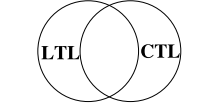
\includegraphics[scale=1.5]{ltlctl.png}
\end{center}
\caption{Izražajnost LTL i CTL}
\label{fig:ltlctlex}
\end{figure}

Algoritam \ref{alg:kaCTL} predstavlja algoritam za proveru modela upotrebom automata i logike stabla izračunavanja i prvi put je u tom obliku prikazan u radu \cite{rozier2011linear} .

\begin{megaalgorithm}
\caption{Algoritam za proveru modela upotrebom automata i logike stabla izračunavanja}\label{alg:kaCTL}
% \DontPrintSemicolon
%  \KwData{$G=(X,U)$ such that $G^{tc}$ is an order.}
 % \KwResult{$G’=(X,V)$ with $V\subseteq U$ such that $G’^{tc}$ is an interval order.}
\textbf{Ulaz: }konacni automat (tranzicioni sistem TS) i CTL formula $\phi$ 

\textbf{Izlaz:} DA ako je TS |= $\phi$; inace, NE i generisan kontraprimer 

\Indp  Definisati model sistema$M$ koji sadrži putanje do svih stanja na osnovu skupa svih zahteva $Prop$

	Neka je $\phi$ CTL formula kojom su zadati zahtevi iz skupa $Prop$ 

	Proveriti da $M \models \phi$

		\Indp Prevesti specifikaciju $\not\phi$ u Büchi automat  $A_{\not\phi}$ i spojiti ga sa modelom sistema $M$ da bi se formirao sistem $A_{M, \not\phi}$
		
		Proveriti da li $A_{M, \not\phi}$ neprazan pretragom putanja koje prihvata $A_{M, \not\phi}$
		
		\textbf{if}  putanja koje prihvata $A_{M, \not\phi}$ postoji
		
		\Indp \textbf{return } NE i putanju kao kontraprimer
		
		\Indm  \textbf{else}	

		\Indp \textbf{return } DA

	\Indm \textbf{fi}
\end{megaalgorithm}

	\section{ESBMC verifikacioni alat}
	\label{sec:ESBMC}

	U dizajnu kompleksnih softverskih sistema više se truda i vremena potroši na
	verifikaciju nego na kontrukciju samog softvera. Verifikacione tehnike  zasnovane na modelima se baziraju na modelima koji opisuju ponašanje sistema na matematički precizan i nedvosmislen način. Ispostavilo se da pre bilo kakvih verifikacionih provera, precizno modelovanje sistema često dovodi do otkrivanja nepravilnosti, nepotpunosti i nelogičnosti u neformalnim specifikacijama sistema. Takvi problemi se obično otkrivaju u kasnim fazama dizajna.Modeli sistema su praćeni algoritmima koji sistematično istražuju sva njihova stanja. To je preduslov za čitav niz tehnika verifikacije polazeći od provera modela preko simulacije do testiranja.
	Provera modela je verifikaciona tehnika koja istražuje sva moguća stanja sistema koristeći brute-force način.
	

ESBMC je kontekstno-ograničeni kontrolor modela za ugrađeni $C\/C++$ softver, baziran na SMT (eng. \emph{satisfiability modulo theory}) rešavaču.  On dozvoljava verifikacionom inženjeru da: 
	\newline
	\begin{enumerate}
	\item Verifikuje jedno- i višenitni softver (sa deljenim promenljivama i međusobnim isključenjem);
	\item Prosuđuje o aritmetičkim prekoračenjima, bezbednosti pokazivača, curenju memorije, granicama nizova, kršenju atomičnosti i redosleda izvršavanja, mrtvim blokadama i utrkivanjima; 
	\item Verifikuje programe koji koriste aritmetiku na nivou bita, pokazivača, struktura, unija i sa fiksnim zarezom.
	\end{enumerate}
	ESBMC ne zahteva od korisnika da komentariše programe sa preduslovima i postuslovima (eng. \emph{pre/post-conditions}), već mu dozvoljava da navede dodatna svojstva koristeći assert-instrukcije, koje se potom kontrolišu. Takođe, obezbeđuje tri pristupa (lenji, snimanje po rasporedu, podaproksimaciju i proširivanje) za kontrolu modela višenitnog softvera. ESBMC može biti pozivan kroz tekstualni komandni interfejs ili podešen putem dodatka za Eclipse. ESBMC obrađuje verifikacione uslove koristeći različite pozadinske teorije i prosleđuje ih direktno u SMT rešavač. Dodatno, ESBMC može da vrati vrednost verifikacionih uslova koristeći.
	\newline
	Podrazumevano, ESBMC proverava da li ima nepravilnosti u samom programskom jeziku, po ISO/ANSI programskom standardu.. Naravno, program može da bude ispravan, ali da ima pogrešnih stvari. Kod takvih slučajeva se dodaju dodatne specifikacije za program koristeći assert instrukcije. 
	\newline
	ESBMC  koristi transformacije  da pretvori program u niz matematičkih ograničenja:
	\begin{enumerate}
	\item Komponente biblioteka su objedinjene u programski tekst.
	\item Kontrola toka se pretvara u jednostavnu GOTO formu.
	\item GOTO program se prevodi u formu  u kojoj se zahteva da je promenljivoj dodeljena vrednost tačno jednom i svaka promenljiva je definisana, pre korišćenja.U ovoj fazi smo se pomerili sa predstavljanja C promenljive u promenljivu koja algebarsku nepoznatu povezuje sa svakim izvršenjem jednog zadatka.
	\item Uvodimo dodatna ograničenja izmedju nepoznatih, koja jedino mogu biti zadovoljena ako program ima grešku.
	\item SMT(eng. \emph{satisfiability modulo theory}) rešavač se pokreće da istraži da li sva ograničenja mogu biti zadovoljena odjednom. Bilo koji uspeh je greška u programu.
	\item Ako SMT solver uspe(program ne prolazi)koristimo njegovo uspešno dodeljivanje promenljive nepoznatoj da zaključimo pogrešan tok programa.
	\end{enumerate}
	Za ovaj primer programa:
	\newline
	\begin{primer}

\begin{verbatim}
	#include  <stdlib.h>  	
	
	int main()
	{
		unsigned int size = nondet_int();
		char *hunk = malloc(size); 
		unsigned int pos = nondet_int(); 
		hunk[pos] = 0;
		return 0;
	}
\end{verbatim}

	Generiše se sledeći izveštaj:
	\newline
	Violated property: file test.c line 10 function main dereference failure: dynamic object upper bound !(\_\_ESBMC\_is\_dynamic[POINTER\_OBJECT(hunk + pos)] \&\& DYNAMIC\_SIZE(hunk + pos) <= POINTER\_OFFSET(hunk) + pos) VERIFICATION FAILED
	\end{primer}


	\subsection{Primena}
	\label{subsec:Primena}

	Verifikacija softvera može imati različite primene.  Najčeća primena alata za verifikaciju je u oblasti  gde je ispravnost programa izrazito važna. 


	\section{Najpoznatiji alati za proveru modela}
\label{sec:NazpM}

Neki od napoznatijih alata za proveru modela su:
\begin{enumerate}
\item ARC
\item BANDERA
\item BLAST
\item CADENCE SMV
\item CADP
\item CBMC
\item CPAchecker
\item CWB-NC
\item DIVINE
\item DREAM
\item DSVerifier
\item EBMC
\item Edinburgh CWB
\item EmbeddedValidator
\item Expander2
\item Fc2Tools
\item GEAR
\item ImProve
\item Java Pathfinder
\item LLBMC
\item LTSA
\item LTSmin
\item MCMAS
\item mCRL2
\item MRMC
\item ompca, OpenMP C Analysis
\item PAT
\item PRISM
\item ProB
\item Reactis Tester
\item RED
\item SAL
\item SATABS
\item SATMC
\item SLMC
\item SPIN
\item Spot
\item TAPAAL
\item TAPAs
\item UPPAAL
\item ROMEO
\end{enumerate}

	\section{Zaključak}
	\label{sec:zakljucak}

Greške su sastavni deo svakog rada i tako se i u računarstvu javljaju kao svuda. Glavni cilj je iste te greške detektovati i otkloniti na vreme, pre nego što postanu pretnja po čitav sistem. Efikasna i formalna verifikacija sistema, na prvom mestu konkurentnih, je jako važna. Temporalne logike imaju jako bitnu ulogu u kreiranju sistema koje se bave istim. Temeljno razumevanje ovih logika je krucijalno za bilo kakvo dalje istraživanje oblasti verifikacije sistema. Ovi sistemi su ekspanziji, njihovom razvoju se sve više i više pridaje na značaju, i teži se ka tome da se svi ulazi/izlazi pokriju i ispravno provere. Naravno i treba posvetiti pažnju već postojećim alatima, kao što je ESBMC, i diskutovati o prednostima i manama istih.


	\addcontentsline{toc}{section}{Literatura}
	\appendix
	\bibliography{seminarski} 
	\bibliographystyle{plain}


	\end{document}
